\subsection{Session flowchart}

\begin{figure}[h!]
\centering
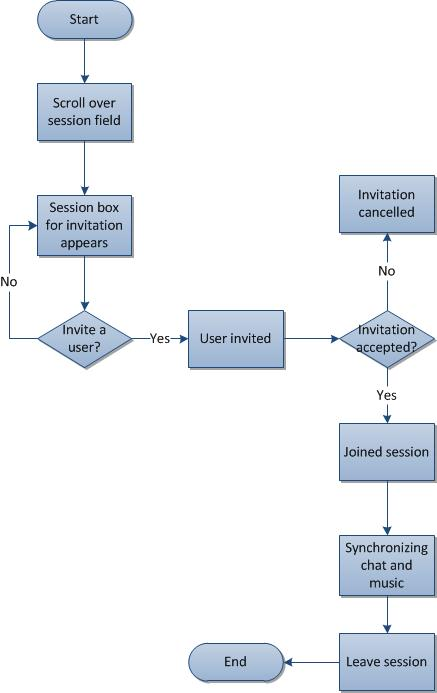
\includegraphics[scale=0.5]{design/figures/session_flowchart}
\caption{Flowchart of session in Movingwhales}
\end{figure}

Here we got the flowchart for session in Movingwhales, lets go through the steps so we can get a better understanding of what is happening in the process.
\begin{description}
\item{Step 1:} We see the field with the name Session in the right side of the site. When we slider over it with the mouse pointer a little window with options appears to the left side of the field, which gets us to.
\item{Step 2:} A little box with options appears fore sessions.
\item{Step 3:} In this step you can choose to invite a user or not. If a user does not get invited then logically nothing happens else we move on to the next step. 
\item{Step 4:} A user has been invited, so he receives a pending invitation then he can do two things. Which leads us to.
\item{Step 5:} Waiting for a response from the invited user. If the invitation gets cancelled we get to step.
\item{Step 6a:} The invitations has been cancelled. Else we get to.
\item{Step 6b:} The invitation has been accepted and so the user joins the session invited to.
\item{Step 7:} The chat and the music in the session get synchronized.
\item{Step 8:} Leaving the session, and so we end up in.
\item{Step 9:} Session ended
\end{description}